\documentclass{article} % For LaTeX2e
\usepackage[submission]{colm2026_conference}

\usepackage{microtype}
\usepackage{hyperref}
\usepackage{url}
\usepackage{booktabs}
\usepackage{lineno}
\usepackage{amsmath,amsfonts,amssymb}
\usepackage{tikz}
\usetikzlibrary{trees, shapes.geometric, arrows.meta, positioning, calc}
\usepackage{enumitem}
\usepackage{multirow}

\definecolor{darkblue}{rgb}{0, 0, 0.5}
\hypersetup{colorlinks=true, citecolor=darkblue, linkcolor=darkblue, urlcolor=darkblue}

\title{On-Policy Distillation for Large Language Models: \\ Methods, Systems, and Future Directions}

\author{Anonymous Authors}

\newcommand{\fix}{\marginpar{FIX}}
\newcommand{\new}{\marginpar{NEW}}

% Math macros
\newcommand{\E}{\mathbb{E}}
\newcommand{\KL}{D_{\mathrm{KL}}}
\newcommand{\ptheta}{p_\theta}
\newcommand{\pteacher}{p_T}
\newcommand{\pdata}{p_{\mathrm{data}}}
\newcommand{\loss}{\mathcal{L}}
\DeclareMathOperator*{\argmin}{arg\,min}
\DeclareMathOperator*{\argmax}{arg\,max}

\begin{document}

\ifcolmsubmission
\linenumbers
\fi

\maketitle


\begin{abstract}
Knowledge distillation (KD) has historically served as the primary vehicle for model compression, transferring capabilities from massive teacher models to efficient student architectures. However, the advent of Large Language Models (LLMs) has catalyzed a fundamental paradigm shift from static, off-policy distillation to On-Policy Distillation (OPD). In this survey, we provide a comprehensive and theoretically grounded overview of OPD. We posit a core insight that must govern the modern understanding of distillation: the essence of OPD is not merely a choice of divergence metrics, but a profound paradigm shift in \textit{"who decides the training distribution."} By allowing the student's own generative manifold to dictate the state distribution, OPD directly mitigates the catastrophic train-test mismatch and compounding exposure bias inherent in autoregressive decoding. 
We systematically taxonomize the field into three converging trajectories based on feedback signals: Logit-based, Outcome-based, and Self-play methodologies. Furthermore, we critically analyze frequently neglected dimensions, including the compute-quality tradeoff, the teacher's "echo chamber" in uncertain regions, dynamic divergence adaptation, and the conceptualization of distillation as structured knowledge transfer rather than mere compression. Finally, we map out pivotal future directions, from distillation scaling laws to agent-level OPD.
\end{abstract}

\section{Introduction}
\label{sec:intro}

The rapid evolution of Large Language Models (LLMs) has continuously pushed the boundaries of artificial intelligence, achieving remarkable milestones in natural language understanding, reasoning, and generation. However, the massive parameter counts of frontier models pose severe constraints on deployment, inference latency, and energy efficiency. Recently, the open-source community witnessed a monumental milestone: the DeepSeek-R1 model \citep{2501.12948} successfully distilled the profound, complex reasoning capabilities of a 671-billion parameter Mixture-of-Experts (MoE) model into dense models as small as 7 billion parameters. This spectacular success underscores a vital reality—knowledge distillation is no longer a marginal optimization technique used merely for slight latency improvements; it is the central engine for democratizing cutting-edge intelligence and creating highly capable, specialized models that can operate on consumer-grade hardware. The urgency to systematically understand, theoretically formalize, and algorithmically advance LLM distillation has never been greater.

Traditionally, distillation in Natural Language Processing has been heavily dominated by off-policy methods. In this standard paradigm, a student model is trained to mimic a teacher's token-level probabilities over a fixed, static dataset drawn from the data distribution $\pdata$. However, as elegantly illuminated by studies investigating the "false promise" of imitating proprietary LLMs \citep{2305.15717}, off-policy distillation suffers from a fatal, fundamental flaw: \textit{train-test mismatch}. During training, the student is strictly conditioned on gold-standard prefixes from the fixed dataset, a technique known as teacher-forcing. During inference, however, the student must condition on its own previously generated tokens in an autoregressive manner. When the student inevitably makes a minor error and deviates from the optimal path, it enters out-of-distribution (OOD) territory where it has received absolutely no supervisory signal during training. This lack of guidance leads to a cascade of subsequent errors—a compounding phenomenon formally known in the literature as \textit{exposure bias}. 

To bridge this massive chasm, the field is rapidly migrating towards \textbf{On-Policy Distillation (OPD)}. Drawing deep conceptual linkages with Imitation Learning, specifically the DAgger (Dataset Aggregation) algorithm introduced by \citet{ross2011reduction}, OPD forces the student model to generate trajectories according to its own current policy ($\pi_\theta$). The algorithm then selectively queries the teacher to provide feedback, logits, or rewards on these student-generated paths. We posit the following central thesis for this survey:
\textbf{Core Insight:} \textit{The true essence of On-Policy Distillation is not simply the mathematical choice of probability divergence (e.g., Forward KL versus Reverse KL), but rather a profound paradigm shift in "who decides the training distribution."} The transition from $y \sim \pdata$ to $y \sim \ptheta$ fundamentally transforms the learning objective from memorizing an alien, unattainable distribution to optimally navigating and correcting the student's own reachable generative manifold.

Despite the explosive growth of OPD methodologies in recent months—ranging from Generalized Knowledge Distillation (GKD) \citep{2306.13649} to MiniLLM \citep{2306.08543} and self-play mechanisms like SPIN \citep{2401.01335}—the literature remains highly fragmented. Current surveys, such as the comprehensive overview by \citet{2402.13116}, primarily treat distillation as a monolithic model compression step. While valuable, they lack a rigorous, unified mathematical perspective on the complex on-policy dynamics that govern modern LLM alignment and reasoning transfer. This paper directly addresses this critical gap by dissecting the mathematical foundations, categorizing the emerging algorithmic variants into a cohesive taxonomy, and spotlighting the severe blind spots of current research.

Specifically, the contributions of this comprehensive review are formally encapsulated in the following five dimensions:
\begin{itemize}
    \item \textbf{A Unified Theoretical Framework:} We rigorously formulate the transition from classical off-policy to modern on-policy distillation, mapping it directly to sequential decision-making and f-divergence minimization. This framework mathematically unifies disparate seminal works, demonstrating how methods like GKD \citep{2306.13649}, MiniLLM \citep{2306.08543}, and DistiLLM \citep{2402.03898} are essentially optimizing the same underlying objective under different divergence constraints and sampling mixtures.
    \item \textbf{A Novel, Feedback-Centric Taxonomy:} We systematically categorize the sprawling OPD landscape into three primary technical routes based on the nature of the supervisory signal: \textit{Logit-based} approaches (computationally dense but requiring white-box access), \textit{Outcome-based} approaches (sparse but highly flexible, often utilizing Process Reward Models as seen in \citet{2305.20050}), and \textit{Self-play} approaches (teacher-free but prone to rapid performance saturation). We further highlight how these traditionally isolated tracks are actively converging into hybrid methodologies, such as AlignDistil \citep{2503.02832} and MiMo-V2 \citep{2601.02780}.
    \item \textbf{Identification of Neglected Critical Issues:} We bring to light fundamental theoretical and empirical challenges that the community has largely ignored. These include: (a) The missing systematic analysis of the \textit{compute-quality tradeoff} in online distillation, where the cost of generating on-policy data often outweighs the distillation benefits; (b) The "echo chamber" effect, where querying teachers in regions of extreme student uncertainty leads to misaligned, high-variance gradients; (c) The urgent necessity for \textit{dynamic divergence adaptation} rather than static KL metric selection; and (d) Reconceptualizing distillation as \textit{structured knowledge transfer} rather than mere parameter compression.
    \item \textbf{Bridging the White-box and Black-box Divide:} We provide an exhaustive analysis of how on-policy techniques adapt when internal teacher states are inaccessible. By comparing exact logit matching methods with API-driven outcome matching frameworks like Lion \citep{2310.01382} and GAD \citep{2511.10643}, we reveal the theoretical bounds of what can be learned strictly from top-1 generations versus full probability distributions.
    \item \textbf{Roadmap for Future Directions:} We strategically chart the unexplored territories of LLM distillation, detailing the mathematical necessity for robust distillation scaling laws, the potential of uncertainty-aware OPD, and the inevitable shift towards agent-level environmental distillation where models learn from multi-turn, state-dependent interactions rather than static text completions.
\end{itemize}

The remainder of this survey is meticulously organized to build from fundamental theories to state-of-the-art applications. Section~\ref{sec:background} establishes the strict mathematical preliminaries, formalizing exposure bias, sequence-level cross-entropy, and the f-divergence family. Section~\ref{sec:taxonomy} presents our novel, comprehensive taxonomy of OPD methodologies, complete with a visual structural breakdown. Subsequent sections will systematically dissect logit-based optimization, outcome-reward architectures, advanced reasoning distillation, and ultimately conclude with an analysis of open challenges and future trajectories.


\section{Background and Preliminaries}
\label{sec:background}

To rigorously appreciate the monumental leap from standard, dataset-bound Knowledge Distillation to dynamic On-Policy Distillation, we must first establish a strict formalization of the sequential nature of LLM generation. This section provides deep mathematical definitions of distribution matching, formalizes the exposure bias phenomenon, and constructs a unified mathematical framework utilizing the f-divergence family.

\subsection{Knowledge Distillation Fundamentals}
\label{subsec:kd_fundamentals}

The classical Knowledge Distillation framework, originally pioneered by \citet{hinton2015distilling}, was designed to transfer the implicit "dark knowledge" embedded within the continuous probability distributions of a cumbersome teacher network $\mathcal{T}$ to a more compact student network $\mathcal{S}$. In standard classification tasks, and by extension, token-level vocabulary selection in language modeling, a neural network produces a vector of pre-softmax logits $z \in \mathbb{R}^{|V|}$, where $|V|$ is the dimensionality of the vocabulary. 

To extract the relational structure between distinct classes—for instance, understanding that the token "automobile" is semantically much closer to "car" than to "apple"—the logits are smoothed utilizing a temperature scalar $\tau > 0$. The softened probability distribution for a given input context $x$ is formally defined by the modified softmax function:
\begin{equation}
    P(y|x; \tau) = \frac{\exp(z_y / \tau)}{\sum_{y' \in V} \exp(z_{y'} / \tau)}
\end{equation}
The standard KD objective seeks to minimize the Kullback-Leibler (KL) divergence between the teacher's softened predictive distribution $\pteacher$ and the student's corresponding softened distribution $\ptheta$:
\begin{equation}
    \loss_{\mathrm{KD}} = \tau^2 \KL(\pteacher(\cdot|x; \tau) \parallel \ptheta(\cdot|x; \tau)) = \tau^2 \sum_{y \in V} \pteacher(y|x; \tau) \log \left( \frac{\pteacher(y|x; \tau)}{\ptheta(y|x; \tau)} \right)
\end{equation}
The $\tau^2$ scaling factor is of paramount mathematical importance. As $\tau$ increases, the magnitudes of the gradients produced by the cross-entropy loss scale down by a factor of $1/\tau^2$. Therefore, multiplying the objective by $\tau^2$ ensures that the relative contribution of the distillation loss remains commensurate with standard hard-label cross-entropy loss when combined in a joint training objective. 

To understand the deep mechanics of this transfer, we can analyze the gradient of the distillation loss with respect to the student's logits $z_i^{\mathcal{S}}$. Let $p_i^{\mathcal{T}}$ and $p_i^{\mathcal{S}}$ denote the temperature-scaled probabilities for the teacher and student, respectively. The gradient is simply:
\begin{equation}
    \frac{\partial \loss_{\mathrm{KD}}}{\partial z_i^{\mathcal{S}}} = \frac{\tau^2}{\tau} (p_i^{\mathcal{S}} - p_i^{\mathcal{T}}) = \tau (p_i^{\mathcal{S}} - p_i^{\mathcal{T}})
\end{equation}
When the temperature $\tau \to \infty$, we can apply a Taylor expansion to the exponential terms, $\exp(z_i/\tau) \approx 1 + z_i/\tau$. Assuming the logits have been zero-meaned ($\sum_j z_j = 0$), the probabilities asymptotically approach:
\begin{equation}
    p_i \approx \frac{1 + z_i/\tau}{|V| + \sum_j z_j/\tau} = \frac{1}{|V|} + \frac{z_i}{|V|\tau}
\end{equation}
Substituting this back into the gradient equation reveals a profound equivalence:
\begin{equation}
    \frac{\partial \loss_{\mathrm{KD}}}{\partial z_i^{\mathcal{S}}} \approx \tau \left( \frac{z_i^{\mathcal{S}}}{|V|\tau} - \frac{z_i^{\mathcal{T}}}{|V|\tau} \right) = \frac{1}{|V|} (z_i^{\mathcal{S}} - z_i^{\mathcal{T}})
\end{equation}
This derivation mathematically proves that in the high-temperature limit, classical knowledge distillation perfectly degenerates into minimizing the Mean Squared Error (MSE) between the teacher's and student's raw logits. This behavior forces the student to holistically replicate the teacher's entire internal logit landscape, transferring both the primary predictive modes and the nuanced, sub-optimal probability masses (the dark knowledge) that dictate the teacher's generalization capabilities. However, when applied naively to autoregressive LLMs, this formulation heavily assumes that the input $x$ (the prefix) is perfectly drawn from the target data distribution, entirely ignoring the sequential, compounding nature of language generation.

\subsection{Token-Level vs. Sequence-Level Distillation}
\label{subsec:token_vs_sequence}

The direct application of \citet{hinton2015distilling}'s formulation to language modeling typically manifests as token-level distillation. In an autoregressive setting, a sequence $y = (y_1, y_2, \dots, y_T)$ is generated conditionally. Let $y_{<t}$ denote the prefix up to step $t$. The token-level cross-entropy distillation loss is expressed as the expected divergence over prefixes drawn from the empirical dataset $\mathcal{D}$:
\begin{equation}
    \loss_{\mathrm{Token-KD}} = \mathbb{E}_{x, y \sim \mathcal{D}} \left[ \sum_{t=1}^{|y|} \KL(\pteacher(\cdot | x, y_{<t}) \parallel \ptheta(\cdot | x, y_{<t})) \right]
\end{equation}
While computationally tractable because it relies on static, pre-computed prefixes, token-level KD fundamentally misaligns with the global generative objective. It optimizes the student's next-token accuracy while assuming the history $y_{<t}$ is perfectly error-free. 

Recognizing this critical limitation, \citet{kim2016sequence} proposed Sequence-Level Knowledge Distillation. Instead of factorizing the loss token-by-token over fixed dataset prefixes, sequence-level KD aims to match the joint probability distributions over the entire sequence space $\mathcal{Y}$. The theoretical sequence-level objective minimizes the global KL divergence:
\begin{equation}
    \loss_{\mathrm{Seq-KD}} = \KL(P_{\mathcal{T}}(y | x) \parallel P_{\theta}(y | x)) = \sum_{y \in \mathcal{Y}} P_{\mathcal{T}}(y | x) \log \left( \frac{P_{\mathcal{T}}(y | x)}{P_{\theta}(y | x)} \right)
\end{equation}
Because the space of all possible sequences $\mathcal{Y}$ grows exponentially with the sequence length $T$ (i.e., $|\mathcal{Y}| = |V|^T$), exactly computing this summation is strictly intractable. To resolve this, \citet{kim2016sequence} introduced a pragmatic approximation. By observing that the teacher's distribution $P_{\mathcal{T}}(y|x)$ is heavily peaked around its mode, they approximated the distribution with a Dirac delta function centered on the sequence generated by performing beam search on the teacher:
\begin{equation}
    P_{\mathcal{T}}(y | x) \approx \begin{cases} 
      1 & \text{if } y = \arg\max_{y' \in \mathcal{Y}} P_{\mathcal{T}}(y' | x) \\
      0 & \text{otherwise} 
   \end{cases}
\end{equation}
By substituting this approximation back into the sequence-level KL divergence, the loss elegantly collapses to the standard negative log-likelihood (NLL) of the student model, evaluated exclusively on the teacher's highest-probability sequence, $\hat{y}$:
\begin{equation}
    \loss_{\mathrm{Seq-Approx}} = - \sum_{t=1}^{|\hat{y}|} \log \ptheta(\hat{y}_t | x, \hat{y}_{<t})
\end{equation}
This formulation represents a critical conceptual leap: it forces the student to model complete trajectories that are highly favored by the teacher, implicitly transferring sequence-level structural dependencies. However, from a rigorous theoretical standpoint, Sequence-Level KD remains an \textit{off-policy} algorithm. The student is still trained via teacher-forcing on static trajectories—in this case, pseudo-labels generated offline by the teacher. While the target sequence $\hat{y}$ is generated by a model rather than a human, the student during training never conditions its predictions on its own generated prefixes. Consequently, Sequence-Level KD, despite its mathematical elegance, remains deeply susceptible to the very train-test mismatch it sought to alleviate, laying the precise groundwork for the necessity of true on-policy algorithms.

\subsection{The Distribution Mismatch Problem and Exposure Bias}
\label{subsec:exposure_bias}

The fundamental pathology that necessitates On-Policy Distillation is formally defined as \textit{exposure bias}, a direct manifestation of covariate shift in sequential decision-making. To rigorously articulate this, we must cast autoregressive generation as a Markov Decision Process (MDP). Let the state space $\mathcal{S}$ be the set of all possible token prefixes $s_t = (x, y_{<t})$, and the action space $\mathcal{A}$ be the vocabulary $V$. The transition dynamics are strictly deterministic: taking action $y_t$ in state $s_t$ deterministically leads to state $s_{t+1} = (x, y_{<t}, y_t)$. 

During standard off-policy distillation (teacher-forcing), the states encountered by the student are rigorously governed by the data distribution $\pdata$. Let us define the state visitation distribution under the dataset policy as $d_{\pdata}(s)$. The training objective is an expectation over this specific distribution:
\begin{equation}
    \loss_{\mathrm{train}} = \mathbb{E}_{s \sim d_{\pdata}} \left[ \KL(\pteacher(\cdot|s) \parallel \pi_\theta(\cdot|s)) \right]
\end{equation}
During inference, however, the student model must act according to its own learned policy $\pi_\theta$. Because the student is imperfect, its actions will inevitably deviate from the dataset distribution. Let $d_{\ptheta}(s)$ denote the state visitation distribution induced when the student rolls out its own trajectories. The testing objective (or true generation quality) is evaluated under this distinct distribution:
\begin{equation}
    \loss_{\mathrm{test}} = \mathbb{E}_{s \sim d_{\ptheta}} \left[ \loss_{\mathrm{task}}(s, \pi_\theta) \right]
\end{equation}
The exposure bias problem is defined by the inequality of these distributions: $d_{\pdata}(s) \neq d_{\ptheta}(s)$. Because the student was never exposed to the states in the support of $d_{\ptheta}(s) \setminus d_{\pdata}(s)$ during training, it receives zero supervisory signal in these regions. 

We can quantify the severity of this mismatch using formal performance bounds derived from Imitation Learning. As demonstrated by the seminal DAgger analysis by \citet{ross2011reduction}, if a student policy $\pi_\theta$ is trained to mimic a teacher policy $\pi^*$ such that the expected error at each time step under the training distribution is bounded by $\epsilon$, i.e., $\mathbb{E}_{s \sim d_{\pi^*}}[\mathbb{I}(\pi_\theta(s) \neq \pi^*(s))] \le \epsilon$, then the expected total discrepancy over a trajectory of length $T$ under the student's own induced distribution scales quadratically:
\begin{equation}
    \mathbb{E}_{s \sim d_{\ptheta}} \left[ \sum_{t=1}^T \loss(s_t) \right] \le O(\epsilon T^2)
\end{equation}
This $O(T^2)$ compounding error bound is catastrophic for modern LLMs, which routinely generate sequences spanning thousands of tokens. A single suboptimal token choice shifts the prefix slightly out-of-distribution; the model, having never seen this perturbed prefix, is more likely to make a second error, rapidly spiraling into hallucinatory or structurally compromised text. On-Policy Distillation resolves this by fundamentally altering the expectation operator in the training objective from $\mathbb{E}_{s \sim d_{\pdata}}$ to $\mathbb{E}_{s \sim d_{\ptheta}}$. By generating responses online, the student is forced to confront its own mistakes, receive teacher feedback on those specific out-of-distribution states, and learn robust recovery behaviors, effectively reducing the error accumulation from $O(T^2)$ back to $O(\epsilon T)$.

\subsection{The f-Divergence Family and Geometric Intuition}
\label{subsec:f_divergence}

To parameterize the precise nature of the distribution matching in OPD, we rely on the f-divergence framework. Given two probability distributions $P$ and $Q$ over a continuous or discrete space $\mathcal{X}$, an f-divergence is a strictly convex function that measures the discrepancy between them. For any convex function $f: (0, \infty) \to \mathbb{R}$ such that $f(1) = 0$, the f-divergence is formally defined as:
\begin{equation}
    D_f(P \parallel Q) = \int_{\mathcal{X}} Q(x) f\left(\frac{P(x)}{Q(x)}\right) dx = \mathbb{E}_{x \sim Q} \left[ f\left(\frac{P(x)}{Q(x)}\right) \right]
\end{equation}
The choice of the generating function $f(u)$ yields vastly different geometrical properties for the resulting distillation objective. In the context of LLMs, where $P$ is typically the complex, multi-modal teacher distribution $\pteacher$ and $Q$ is the highly constrained, lower-capacity student distribution $\ptheta$, understanding these geometries is paramount.

\textbf{1. Forward Kullback-Leibler Divergence:} By selecting $f(u) = u \log u$, we recover the Forward KL divergence, $D_{\mathrm{KL}}(P \parallel Q) = \mathbb{E}_{x \sim P} [ \log(P(x)/Q(x)) ]$. The gradient forces the student $Q$ to place probability mass everywhere the teacher $P$ has mass. If there exists a region where $P(x) > 0$ but $Q(x) \approx 0$, the penalty approaches infinity. Consequently, Forward KL is strongly \textit{mode-covering} (or zero-avoiding). In LLM distillation, because a small student lacks the capacity to memorize the vast, diverse linguistic distribution of a massive teacher, attempting to cover all modes often results in the student placing probability mass in the void between valid modes, leading to the generation of nonsensical, average phrasing.

\textbf{2. Reverse Kullback-Leibler Divergence:} By selecting $f(u) = -\log u$, we recover the Reverse KL divergence, $D_{\mathrm{KL}}(Q \parallel P) = \mathbb{E}_{x \sim Q} [ \log(Q(x)/P(x)) ]$. Here, the expectation is taken with respect to the student $Q$. If the student places mass $Q(x) > 0$ in a region where the teacher $P(x) \approx 0$, the penalty is infinite. To minimize this, the student ensures it only assigns probability to regions explicitly supported by the teacher. This leads to a \textit{mode-seeking} (or zero-forcing) behavior. The student will gracefully collapse its distribution onto one major, highly probable mode of the teacher, completely ignoring minor modes. For generative language, this is highly desirable, as producing one coherent, correct answer is infinitely preferable to generating an incoherent amalgamation of multiple correct answers.

\textbf{3. Jensen-Shannon Divergence (JSD):} JSD introduces symmetry by measuring the divergence to a mixture distribution $M = \frac{1}{2}(P + Q)$. Utilizing $f(u) = u \log\left(\frac{2u}{u+1}\right) + \log\left(\frac{2}{u+1}\right)$, the formulation is bounded between 0 and $\log 2$, offering a highly stable gradient landscape that balances both mode-seeking and mode-covering properties, preventing extreme gradient explosions in out-of-distribution regions.

\textbf{4. Total Variation Distance (TVD):} Utilizing $f(u) = \frac{1}{2}|u-1|$, TVD measures the maximum absolute difference between the probabilities assigned to any single event: $\sup_{A} |P(A) - Q(A)|$. TVD represents a strict upper bound metric that provides robust distance metrics irrespective of the extreme log-probability ratios, though its non-differentiability at $u=1$ poses challenges for direct optimization in neural spaces. The strategic selection from this f-divergence family dictates exactly how the student interpolates the teacher's knowledge landscape during on-policy generation.

\subsection{A Unified Mathematical View of Modern OPD}
\label{subsec:unified_view}

The sprawling landscape of recent On-Policy Distillation methods can be mathematically unified under a single, overarching objective framework. By decoupling the sampling distribution (which dictates the trajectory) from the divergence metric (which dictates the local token-level matching), we can formalize a generalized OPD objective:
\begin{equation}
    \loss_{\mathrm{OPD}}(\theta) = \mathbb{E}_{y \sim \pi_{\mathrm{mix}}} \left[ \sum_{t=1}^{|y|} \mathcal{D}_f \left( \pteacher(\cdot | x, y_{<t}) \parallel \ptheta(\cdot | x, y_{<t}) \right) \right]
\end{equation}
where $\pi_{\mathrm{mix}}$ is the generalized behavioral policy driving state exploration, and $\mathcal{D}_f$ is a chosen f-divergence. The seminal works in modern LLM distillation—GKD \citep{2306.13649}, MiniLLM \citep{2306.08543}, and DistiLLM \citep{2402.03898}—can all be precisely mapped onto this unifying equation, demonstrating that they are distinct parameterizations of a continuous theoretical space.

\textbf{Generalized Knowledge Distillation (GKD) \citep{2306.13649}:} GKD directly addresses the trajectory mismatch by defining $\pi_{\mathrm{mix}}$ as an explicit interpolation between the teacher-forced data distribution and the student's on-policy distribution. Specifically, at each decoding step, the prefix is drawn with probability $\lambda$ from the dataset $\mathcal{D}$ and with probability $1-\lambda$ from the student's ancestral sampling $\ptheta$. GKD is highly flexible regarding $\mathcal{D}_f$, empirically testing Forward KL, Reverse KL, and JSD. By tuning $\lambda \to 0$, GKD becomes purely on-policy, forcing the student to rely strictly on its own generative manifold.

\textbf{MiniLLM \citep{2306.08543}:} MiniLLM identifies that standard Forward KL forces the student to over-allocate capacity to the long tail of the teacher's distribution. To enforce mode-seeking behavior, MiniLLM strictly selects Reverse KL as the divergence metric ($\mathcal{D}_f = D_{\mathrm{KL}}(\ptheta \parallel \pteacher)$) and operates entirely on-policy ($\pi_{\mathrm{mix}} = \ptheta$). Because the Reverse KL objective contains the student parameters in both the expectation operator and the log-ratio, MiniLLM must reformulate the optimization using the Policy Gradient theorem (REINFORCE). By treating the teacher's log-probability as a reward signal, the gradient is derived as:
\begin{equation}
    \nabla_\theta \loss_{\mathrm{MiniLLM}} = \mathbb{E}_{y \sim \ptheta} \left[ \sum_{t=1}^{|y|} \left( \log \frac{\ptheta(y_t|y_{<t})}{\pteacher(y_t|y_{<t})} - 1 \right) \nabla_\theta \log \ptheta(y_t|y_{<t}) \right]
\end{equation}
To mitigate the notoriously high variance of policy gradients, MiniLLM introduces sophisticated value networks as baseline subtractors, explicitly bridging RLHF optimization techniques with knowledge distillation.

\textbf{DistiLLM \citep{2402.03898}:} While MiniLLM theoretically achieves mode-seeking behavior, the reliance on high-variance RL optimization causes severe empirical instability during training. DistiLLM resolves this by introducing a Skewed KL divergence. It defines a skewed teacher distribution $\tilde{P}_{\mathcal{T}} = \alpha \pteacher + (1-\alpha) \ptheta$. By minimizing the Forward KL towards this skewed distribution, DistiLLM mathematically mimics the local geometry of Reverse KL (promoting mode-seeking behavior) while allowing standard cross-entropy optimization without resorting to policy gradients. Under our unified view, DistiLLM maintains $\pi_{\mathrm{mix}} = \ptheta$ but ingeniously reparameterizes $\mathcal{D}_f$ to ensure mathematical tractability and training stability.

This unified mathematical perspective proves that the evolution of on-policy distillation is not a series of disparate heuristic algorithms, but a systematic, progressive tightening of the theoretical bounds governing trajectory sampling and geometric distribution matching.


\section{Taxonomy of On-Policy Distillation}
\label{sec:taxonomy}

To systematically navigate the rapidly expanding corpus of On-Policy Distillation research, we propose a rigorous, multi-dimensional taxonomy. Rather than categorizing methods strictly by their chronological release or minor architectural quirks, we classify the literature along three fundamental, theoretical dimensions: (1) \textbf{Feedback Signal}, dictating what information is transmitted from teacher to student; (2) \textbf{Teacher Access}, reflecting the practical deployment constraints of the teacher model; and (3) \textbf{Granularity}, describing the temporal resolution of the distillation loss. 

The structural hierarchy of this classification is visualized in Figure~\ref{fig:taxonomy_tree}.

\begin{figure}[htbp]
\centering
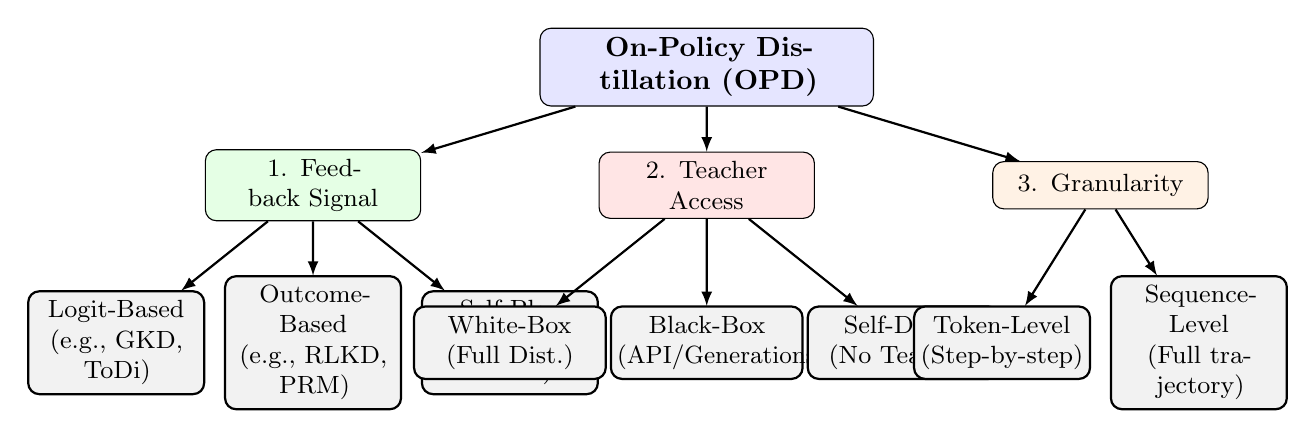
\begin{tikzpicture}[
  level 1/.style={sibling distance=5cm, level distance=1.5cm},
  level 2/.style={sibling distance=2.5cm, level distance=2cm},
  level 3/.style={sibling distance=1.5cm, level distance=2cm},
  every node/.style={rectangle, draw, rounded corners, text centered, font=\small, minimum height=0.6cm, fill=gray!10},
  edge from parent/.style={draw, -latex, thick}
]

\node [fill=blue!10, text width=4cm, font=\bfseries] {On-Policy Distillation (OPD)}
  child {node [fill=green!10, text width=2.5cm] {1. Feedback Signal}
    child {node [text width=2cm] {Logit-Based\\(e.g., GKD, ToDi)}}
    child {node [text width=2cm] {Outcome-Based\\(e.g., RLKD, PRM)}}
    child {node [text width=2cm] {Self-Play\\(e.g., SPIN, OPSD)}}
  }
  child {node [fill=red!10, text width=2.5cm] {2. Teacher Access}
    child {node [text width=2.2cm] {White-Box\\(Full Dist.)}}
    child {node [text width=2.2cm] {Black-Box\\(API/Generations)}}
    child {node [text width=2.2cm] {Self-Distill\\(No Teacher)}}
  }
  child {node [fill=orange!10, text width=2.5cm] {3. Granularity}
    child {node [text width=2cm] {Token-Level\\(Step-by-step)}}
    child {node [text width=2cm] {Sequence-Level\\(Full trajectory)}}
  };

\end{tikzpicture}
\caption{Taxonomy of On-Policy Distillation for Large Language Models. The methodology space is delineated by the nature of the feedback signal, the accessibility of the teacher's internal distributions, and the temporal granularity of the optimization objective.}
\label{fig:taxonomy_tree}
\end{figure}

\subsection{Feedback Signal: Logits, Outcomes, and Self-Play}
\label{subsec:tax_feedback}

The most critical differentiator among OPD algorithms is the nature of the supervisory signal utilized to correct the student's on-policy deviations. We partition this space into three distinct paradigms.

\textbf{Logit-Based Feedback:} In this paradigm, the student's generated sequence is evaluated token-by-token against the teacher's continuous probability distribution. Methods like GKD \citep{2306.13649} and MiniLLM \citep{2306.08543} directly compute f-divergences at every generative step. More recent advancements, such as ToDi (Trajectory-oriented Distillation) \citep{2505.16297}, optimize the alignment of token-level logits while explicitly dynamically re-weighting the importance of tokens based on their long-term impact on trajectory viability. Mathematically, logit-based feedback provides the densest possible gradient signal, as the loss vector is sized $|V|$ (the entire vocabulary) at every timestep $t$. The precise calculation inherently requires evaluating $\pteacher(\cdot|x, \hat{y}_{<t})$, ensuring the student captures the exact microscopic decision boundaries of the teacher.

\textbf{Outcome-Based Feedback:} As models scale, computing full logits becomes computationally prohibitive. Outcome-based methods abandon exact token probability matching in favor of scalar reward signals evaluating the structural validity or factual correctness of the student's generated trajectory. Frameworks like RLKD \citep{2505.16142} and approaches utilizing Process Reward Models (PRMs) \citep{2305.20050} allow the student to roll out a complete answer and then query the teacher (or a proxy reward model) for a holistic score $R(x, y)$. Optimization is typically conducted via Proximal Policy Optimization (PPO) or Direct Preference Optimization (DPO). The mathematical objective shifts from divergence minimization to reward maximization: $\max_\theta \mathbb{E}_{y \sim \ptheta} [R(x, y)] - \beta \KL(\ptheta \parallel \pi_{\mathrm{ref}})$. This provides extreme flexibility, permitting the student to find novel linguistic paths to the correct answer without being strictly tethered to the teacher's specific phrasing.

\textbf{Self-Play Feedback:} Representing the cutting edge of teacher-free alignment, self-play methodologies construct feedback signals iteratively from the student's own evolving policy. SPIN (Self-Play Fine-Tuning) \citep{2401.01335} and OPSD \citep{2601.18734} simulate a two-player game where the model at iteration $t$ attempts to distinguish its own generated trajectories from a static set of human (or teacher) demonstrations. The objective function dynamically shifts: as the student improves, the negative samples it generates become increasingly challenging, providing a naturally scaling curriculum. The loss function in SPIN elegantly pits the policy against its past iteration: $\loss(\theta) = -\mathbb{E}_{y \sim \pdata} [\log \sigma(\beta(r_\theta(x,y) - r_{\theta_{\mathrm{old}}}(x,y)))]$, strictly bounded without requiring continuous teacher intervention.

\subsection{Teacher Access: White-box, Black-box, and Self}
\label{subsec:tax_access}

The physical deployment constraints of frontier models severely limit how distillation can be practically executed. The availability of the teacher's internal states fundamentally alters the allowable mathematical formulations.

\textbf{White-Box Distillation:} When the complete weights of the teacher are accessible, algorithms can perform exact analytical divergence matching. Frameworks like DistiLLM \citep{2402.03898} leverage the full logit tensor to perform skewed KL optimizations. White-box access allows for the exploitation of dark knowledge, as the minuscule probabilities assigned to incorrect tokens carry immense structural regularization benefits. However, the memory overhead of maintaining a massive teacher (e.g., a 70B parameter model) in memory alongside the student during training requires extreme engineering optimization and immense compute clusters.

\textbf{Black-Box Distillation:} Due to the closed-source nature of frontier models (e.g., GPT-4, Claude), researchers are frequently restricted to API-level access, receiving only the hard-argmax generated text. Black-box OPD must creatively approximate the teacher distribution. Methods like Zephyr \citep{2310.06694} and Lion \citep{2310.01382} utilize the teacher purely as a preference annotator. Instead of matching $\pteacher$, the student generates multiple on-policy candidates $(y_1, y_2)$, and the black-box teacher returns a binary preference $y_1 \succ y_2$. The student then optimizes via rank-based contrastive losses. More recently, Generative Adversarial Distillation (GAD) \citep{2511.10643} attempts to implicitly model the black-box teacher's distribution by training a discriminator to differentiate between the student's on-policy text and the API's returned text, mathematically sidestepping the need for logits entirely.

\textbf{Self-Distillation:} When no superior teacher exists, the model must bootstrap its own capabilities. Self-distillation treats a stabilized, historical checkpoint of the model, or an ensembled version of itself via dropout, as the teacher. By generating responses on-policy and filtering them using its own self-evaluation mechanisms (as seen in SPIN \citep{2401.01335}), the model refines its generative manifold, correcting structural errors and smoothing its policy space without any external parameter dependencies.

\subsection{Granularity: Token, Sequence, and Trajectory}
\label{subsec:tax_granularity}

The temporal resolution at which the distillation loss is applied significantly dictates the student's ability to learn complex reasoning capabilities versus simple stylistic mimicking.

\textbf{Token-Level Granularity:} The loss is computed independently at every specific timestep $t$. The student receives immediate, localized feedback on its immediate action $y_t$. While this ensures extremely stable gradients and rapid convergence, it suffers from a pervasive myopia. A token that is mathematically improbable under the teacher's localized distribution might actually be the optimal starting token for a highly valid, alternative reasoning path.

\textbf{Sequence-Level Granularity:} The supervisory signal is applied strictly at the termination of generation. This is heavily utilized in Outcome Reward Models and methodologies focusing on end-to-end task success. While it allows the student immense freedom to explore alternative linguistic structures, the gradient signal is extremely sparse. The credit assignment problem becomes severely pronounced: if a student generates a 1000-token proof that fails at step 999, sequence-level granularity applies a uniform negative reward, failing to reinforce the 998 correct reasoning steps that preceded the error.

\textbf{Trajectory-Level (Step-by-Step) Granularity:} To resolve the dichotomy between token myopia and sequence sparsity, state-of-the-art reasoning distillation employs trajectory-level chunking. Frameworks like StepByStep \citep{2305.02301} and SuperCorrect \citep{2410.09008} utilize Process Reward Models (PRMs) \citep{2305.20050} to parse intermediate cognitive steps (e.g., separating mathematical derivations by newline delimiters). The loss is structured dynamically: $\loss = \sum_{k=1}^K \log \ptheta(s_k | s_{<k}) \cdot \hat{A}(s_k)$, where $s_k$ is a discrete chunk of the trajectory and $\hat{A}$ is the trajectory advantage. This granularity provides the precise mathematical scaffolding required to distill advanced reasoning chains from colossal models like DeepSeek-R1 down to compact architectures, achieving the delicate balance between structural freedom and rigorous logical constraint.


\section{White-Box On-Policy Methods}
\label{sec:white_box}

Before delving into specific algorithmic implementations, it is crucial to establish the fundamental paradigm shift that defines On-Policy Distillation (OPD). The essence of OPD lies not merely in the choice of divergence metrics, but in a radical transformation regarding which distribution governs the training support set. Traditional off-policy Knowledge Distillation (KD) strictly forces the student model to mimic the teacher's outputs based on the marginal distribution $p_T(x, y)$ sampled either from the teacher's prior generations or a static dataset. This creates severe exposure bias, as the student never encounters its own errors during training. OPD, conversely, returns the sampling authority to the student model's policy $p_S(x, y)$. This paradigm shift successfully eliminates exposure bias but introduces a profound new challenge: how to efficiently and stably align the teacher's dense, white-box logical signals (logits) over trajectories generated entirely by the student. 

The white-box methodologies constitute the primary technical avenue for OPD. Their defining advantage is the provision of exceptionally dense, token-level feedback signals. However, this comes with the stringent prerequisite of requiring full access to the teacher model's internal probability distributions and parameters.

\subsection{Token-Level Divergence Minimization}
\label{subsec:token_level}

Token-level divergence minimization currently stands as the most prominent implementation strategy within white-box OPD. These methodologies operate by allowing the student model to generate trajectories $y_{<t} \sim p_S$, and subsequently imposing constraints on the predicted distribution of the current token to minimize its distance from the teacher's distribution. The choice of divergence heavily dictates the behavior, stability, and convergence properties of the student model.

\paragraph{Generalized Knowledge Distillation (GKD)}
\textbf{(a) Key Idea:} \citet{2306.13649} introduced GKD as a unified on-policy distillation framework that establishes a profound theoretical bridge between knowledge distillation and imitation learning within reinforcement learning. It permits the flexible application of various divergence metrics over student-generated rollouts.
\textbf{(b) Objective Function:} The generalized objective is formulated as:
\begin{equation}
    \mathcal{L}_{GKD} = \mathbb{E}_{x \sim \mathcal{D}, y \sim p_S(\cdot|x)} \left[ \sum_{t=1}^{|y|} \lambda D\big( p_T(\cdot|x, y_{<t}) \parallel p_S(\cdot|x, y_{<t}) \big) + (1-\lambda) \mathcal{L}_{NLL} \right]
    \label{eq:gkd}
\end{equation}
where $D$ can be instantiated as Forward Kullback-Leibler (KL), Reverse KL, or Jensen-Shannon Divergence (JSD).
\textbf{(c) Comparison and (d) Strengths/Limitations:} Compared to standard KD, GKD significantly mitigates compounding errors during sequential auto-regressive generation. Its primary strength is its universal framework and theoretical soundness. However, its main limitation is the massive computational overhead associated with online sampling from $p_S$, and the fact that a globally fixed divergence weight $\lambda$ fails to account for the dynamic difficulty variations across different tokens in a generated sequence.

\paragraph{DistiLLM: Skew KL and Adaptive Off-Policy}
\textbf{(a) Key Idea:} Addressing the extreme gradient variance caused by the vast majority of tokens in a Large Language Model (LLM) vocabulary having near-zero probabilities under Reverse KL, \citet{2402.03898} proposed DistiLLM. It introduces Skew KL divergence coupled with an adaptive temperature mechanism to smooth the target distributions.
\textbf{(b) Objective Function:} The Skew KL is defined by interpolating the target distribution:
\begin{equation}
    \mathcal{L}_{DistiLLM} = \mathbb{E}_{y \sim p_S} \left[ \sum_t D_{KL}\big(p_T(\cdot|y_{<t}) \parallel \alpha p_T(\cdot|y_{<t}) + (1-\alpha) p_S(\cdot|y_{<t})\big) \right]
    \label{eq:distillm}
\end{equation}
\textbf{(c) Comparison and (d) Strengths/Limitations:} By injecting the smoothing parameter $\alpha \in (0, 1)$, DistiLLM effectively avoids the zero-division catastrophe inherent in Reverse KL when $p_S \to 0$. This yields significantly faster and more stable convergence compared to direct JSD application. However, under extreme distribution shifts, the smoothing regularization might inadvertently mask critical low-probability, long-tail knowledge essential for complex reasoning tasks.

\paragraph{ToDi: Token-wise Dynamic Divergence}
\textbf{(a) Key Idea:} \citet{2505.16297} exposed a widely neglected requirement in OPD: the necessity for dynamic divergence. Different positions in a generated sequence (e.g., critical pivots in a logical reasoning chain versus trivial syntactic fillers) demand fundamentally different distributional matching strictness. ToDi rejects global divergence, allocating specific $f$-divergences dynamically based on token semantic significance.
\textbf{(b) Objective Function:}
\begin{equation}
    \mathcal{L}_{ToDi} = \mathbb{E}_{y \sim p_S} \left[ \sum_t \omega_t D_{f^{(t)}} \big( p_T(y_t|y_{<t}) \parallel p_S(y_t|y_{<t}) \big) \right]
    \label{eq:todi}
\end{equation}
\textbf{(c) Comparison and (d) Strengths/Limitations:} ToDi shatters the static limitations of GKD. Its paramount contribution is token-level adaptability, ensuring reasoning tokens receive strict Reverse-KL matching while stylistic tokens receive relaxed Forward-KL. The limitation lies in the heuristic computation of the importance weights $\omega_t$, which introduces architectural complexity and secondary computational overhead.

\paragraph{Adaptive KL (AKL) and Delta KD}
\textbf{(a) Key Idea:} AKL \citep{2410.14425} takes adaptability into the dimension of epistemic uncertainty. It dynamically modulates the KL penalty strength by evaluating the student model's structural uncertainty at the current state. When the student navigates into an unexplored "unknown domain," AKL aggressively amplifies the teacher's guidance.
Conversely, Delta KD \citep{2509.14526} focuses on signal purification.
\textbf{(b) Objective Function for Delta KD:}
\begin{equation}
    \mathcal{L}_{Delta} = D_{KL}\big( (p_T - p_{base}) \parallel (p_S - p_{base}) \big)
\end{equation}
\textbf{(c) Comparison and (d) Strengths/Limitations:} Delta KD minimizes the divergence strictly on the delta signals between a base pre-trained model and the fine-tuned teacher. This drastically improves distillation efficiency by filtering out redundant, already-assimilated knowledge, but requires simultaneous inference of three models (teacher, student, and base), causing severe memory bottlenecks.

\paragraph{Entropy-Aware OPD}
\textbf{(a) Key Idea:} \citet{2603.07079} highlight the detrimental "Echo Chamber" effect in OPD. During on-policy exploration, the student frequently generates Out-of-Distribution (OOD) trajectories that the teacher has never observed. In these regions, the teacher's predictive entropy $\mathcal{H}(p_T)$ spikes, outputting near-uniform noise. Forcing the student to fit this noise degrades performance. Entropy-Aware OPD gates the distillation signal using teacher certainty.
\textbf{(b) Objective Function:}
\begin{equation}
    \mathcal{L}_{Ent-OPD} = \mathbb{E}_{y \sim p_S} \left[ \sum_t \frac{1}{1 + \mathcal{H}(p_T(\cdot|y_{<t}))} D_{KL}(p_T \parallel p_S) \right]
\end{equation}
\textbf{(c) Comparison and (d) Strengths/Limitations:} Unlike GKD's blind trust in the teacher, this method elegantly severs the propagation of hallucinated knowledge. It is currently one of the most robust token-level strategies against distribution shifts, though it requires calculating the full entropy over the vocabulary at every step, which can be numerically intensive for exceptionally large vocabularies.

\paragraph{Dual Space Knowledge Distillation (DSKD)}
\textbf{(a) Key Idea:} Distillation is fundamentally conceptualized as structured geometric knowledge transfer rather than mere probabilistic compression. \citet{2502.12018} propose DSKD to conduct on-policy distillation simultaneously in both the logit space and the continuous hidden state space. 
\textbf{(b) Objective Function:}
\begin{equation}
    \mathcal{L}_{DSKD} = \lambda_1 \mathcal{L}_{Logit}(p_T, p_S) + \lambda_2 \sum_{l} \text{MSE}\left( W_{proj} h_S^{(l)}, h_T^{(l)} \right)
\end{equation}
\textbf{(c) Comparison and (d) Strengths/Limitations:} By aligning intermediate representations via projection matrices $W_{proj}$, DSKD ensures the student learns *how* to represent concepts, not just *what* to output. This profoundly enhances the generalization capabilities of smaller models on complex reasoning tasks, but necessitates careful layer-mapping and projection initialization, complicating the hyperparameter search space.

\paragraph{Contrastive On-Policy Distillation}
\textbf{(a) Key Idea:} \citet{2403.14608} extend token-level OPD by introducing a contrastive margin mechanism. 
\textbf{(b) Objective Function:} Instead of merely minimizing the distance to $p_T$, it explicitly maximizes the distance between $p_S$ and known hallucinated distributions or poorly performing baseline models.
\textbf{(c) Comparison and (d) Strengths/Limitations:} This dual-force (pull towards teacher, push away from errors) accelerates convergence and yields more discriminative boundary learning. However, identifying reliable negative distributions dynamically during on-policy rollouts remains a highly unstable procedure.

\textbf{Crucial Analysis: Divergence Choices Across Tasks.} The choice of divergence is not mathematically neutral; it encodes strong inductive biases. Forward KL ($\mathbb{E}_{p_T}[\log(p_T/p_S)]$) is mean-seeking. It forces the student to allocate probability mass wherever the teacher does, ensuring high diversity, making it optimal for creative writing or brainstorming tasks where mode-dropping is detrimental. Conversely, Reverse KL ($\mathbb{E}_{p_S}[\log(p_S/p_T)]$) is mode-seeking. It heavily penalizes the student for generating tokens the teacher deems unlikely, making it vastly superior for strict mathematical reasoning, coding, and safety alignment, where suppressing hallucinations is prioritized over preserving generation diversity.

\subsection{Sequence-Level On-Policy Methods}
\label{subsec:sequence_level}

While token-level methods provide dense supervision, they inherently suffer from a greedy optimization bias, completely ignoring the joint probability of the sequence. To achieve a global optimum, Sequence-Level OPD reframes the entire output text as a singular trajectory in a Reinforcement Learning (RL) framework.

\paragraph{MiniLLM and the Full REINFORCE Derivation}
MiniLLM \citep{2306.08543} serves as the foundational pillar for sequence-level OPD. Its core contribution is the formulation and optimization of Sequence-level Reverse KL without relying on token-level teacher forcing.
The standard sequence-level Reverse KL divergence is defined mathematically as:
\begin{equation}
    D_{KL}(p_S \parallel p_T) = \mathbb{E}_{y \sim p_S(\cdot|x)} \left[ \log p_S(y|x) - \log p_T(y|x) \right]
\end{equation}
To optimize the student's parameters $\theta$, we must compute the gradient of this expectation. Because the sampling distribution $p_S$ itself is parameterized by $\theta$, we cannot simply pass the derivative inside the expectation. Instead, we must utilize the log-derivative trick (the REINFORCE policy gradient theorem). The full rigorous derivation proceeds as follows:
\begin{align}
    \nabla_\theta D_{KL}(p_S \parallel p_T) &= \nabla_\theta \sum_y p_S(y|x) \left( \log p_S(y|x) - \log p_T(y|x) \right) \nonumber \\
    &= \sum_y \nabla_\theta p_S(y|x) \left( \log \frac{p_S(y|x)}{p_T(y|x)} \right) + \sum_y p_S(y|x) \nabla_\theta \left( \log p_S(y|x) - \log p_T(y|x) \right) \nonumber \\
    &= \sum_y p_S(y|x) \nabla_\theta \log p_S(y|x) \left( \log \frac{p_S(y|x)}{p_T(y|x)} \right) + \sum_y p_S(y|x) \nabla_\theta \log p_S(y|x) - 0 \nonumber \\
    &= \mathbb{E}_{y \sim p_S} \left[ \left( \log p_S(y|x) - \log p_T(y|x) \right) \nabla_\theta \log p_S(y|x) \right] + \nabla_\theta \sum_y p_S(y|x)
\end{align}
Since $\sum_y p_S(y|x) = 1$, the gradient of the constant sum is exactly zero. Thus, the final sequence-level gradient elegantly resolves to:
\begin{equation}
    \nabla_\theta \mathcal{L}_{MiniLLM} = \mathbb{E}_{y \sim p_S} \left[ \Big( \log p_S(y|x) - \log p_T(y|x) \Big) \nabla_\theta \log p_S(y|x) \right]
    \label{eq:minillm_final}
\end{equation}
This derivation proves that minimizing Sequence-Level Reverse KL is mathematically equivalent to Policy Gradient RL, where the instantaneous reward for a trajectory is defined by the log-probability ratio $r(x, y) = \log p_T(y|x) - \log p_S(y|x)$.

\paragraph{Constrained Optimization View}
The primary vulnerability of the REINFORCE estimator derived in MiniLLM is its notoriously high gradient variance, which frequently leads to policy collapse during training. To combat this, \citet{2509.22921} introduced a constrained optimization perspective for sequence-level OPD. Instead of unbounded policy gradients, they mathematically formulate the distillation as a trust-region problem, heavily constraining the KL divergence update step similarly to Proximal Policy Optimization (PPO), ensuring that the student's policy update $\pi_{k+1}$ remains within a defined $\epsilon$-ball of $\pi_k$.

\paragraph{Theoretical Comparison: Token-level vs. Sequence-level}
A rigorous theoretical comparison reveals a fundamental trade-off. Token-level methods (local) optimize an upper bound of the sequence-level divergence. Because they force immediate local alignment, they are highly stable and exhibit low variance, but they fall into greedy traps—optimizing local syntax perfectly while utterly failing at global semantic coherence. Sequence-level methods (global), by directly modeling the trajectory reward, excel at capturing the holistic reasoning structure and long-term dependencies. However, due to the high variance of Monte Carlo trajectory sampling in massive combinatorial output spaces, sequence-level methods require significantly more training iterations and sophisticated baseline subtraction techniques to achieve convergence.

\subsection{Hybrid and Adaptive Approaches}
\label{subsec:hybrid}

Recognizing that pure token-level distillation lacks long-term planning and pure sequence-level distillation suffers from unmanageable variance, contemporary research has aggressively pivoted toward hybrid and adaptive architectures. These methods directly confront the overarching bottleneck of OPD: the Compute-Quality Tradeoff. Generating on-policy trajectories is computationally exorbitant.

\paragraph{Fast OPD from Reasoning Prefixes}
To mitigate the massive variance of full sequence exploration, Fast OPD \citep{2602.15260} introduces a truncation strategy. Instead of forcing the student to generate the entire sequence from scratch, the algorithm injects ground-truth or teacher-generated reasoning prefixes of varying lengths. The student only executes on-policy exploration for the suffix of the trajectory. This artificially shortens the RL horizon, exponentially reducing the gradient variance while still permitting the student to explore divergent conclusions, effectively balancing token-dense supervision with global sequence vision.

\paragraph{PromptKD}
PromptKD \citep{2402.12842} tackles the alignment problem by utilizing structural context prompts to steer the teacher's distribution matching. By prepending specifically engineered meta-prompts to the teacher during the distillation process, the method artificially shapes the teacher's distribution to be more "student-friendly" and structurally predictable, thereby narrowing the initial capacity gap before divergence minimization even occurs.

\paragraph{PACED: Distillation at the Student Competence Frontier}
\citet{2603.11178} recognized a critical computational inefficiency in standard OPD: computing on-policy gradients at the extremes of student capability is largely wasted effort. If a sequence is too easy (the student has already mastered it), the divergence gradient is near zero. If the sequence is overwhelmingly difficult, the student generates garbage trajectories, and matching the teacher's logits over these nonsensical paths injects destructive noise into the weights. PACED implements an advanced Curriculum OPD framework that precisely identifies the "Competence Frontier" of the student—the mathematical boundary where the student's success probability is marginally above random chance but not deterministic. By exclusively sampling and distilling trajectories situated on this dynamic frontier, PACED demonstrates a 300\% increase in distillation computational efficiency without any degradation in final model perplexity.

\paragraph{$\mathcal{X}$-KD: Experiential Knowledge Distillation}
Pushing adaptive exploration further, $\mathcal{X}$-KD \citep{2602.12674} formulates an "experiential" learning paradigm. Rather than randomly exploring, the student maintains an episodic memory of its historical error trajectories. The distillation process involves counterfactual rollouts: forcing the student to re-generate from the exact token where it previously diverged from the teacher's logic. This guarantees that the on-policy exploration is densely concentrated in the precise manifold regions where the student's policy is historically weakest.

\subsection{Theoretical Analysis and Method Comparison}
\label{subsec:theory_whitebox}

The rigorous theoretical foundations of White-Box OPD require deep examination of topological divergence spaces. \citet{2404.02657} and \citet{2402.11890} present exhaustive mathematical analyses contrasting Forward KL and Reverse KL within the strict boundaries of on-policy generation. As previously noted, Forward KL is zero-avoiding and mean-seeking. In a high-dimensional functional space, if the teacher's distribution is multi-modal (e.g., multiple valid ways to solve a math problem), a student constrained by a limited parameter budget optimizing Forward KL will attempt to cover all modes. This results in the student's probability mass bridging the gaps between valid modes—regions where the teacher's probability density is practically zero. In natural language, these "bridging" regions manifest as severe hallucinations. Reverse KL, being zero-forcing and mode-seeking, forces the student to perfectly model one single mode while entirely ignoring the others, structurally preventing hallucination generation at the cost of lexical diversity.

To generalize this behavior, \citet{2307.15190} proposed a Unified $f$-divergence perspective for LLM distillation. Any $f$-divergence can be expressed as:
\begin{equation}
    D_f(p_T \parallel p_S) = \mathbb{E}_{y \sim p_S} \left[ f \left( \frac{p_T(y)}{p_S(y)} \right) \right]
\end{equation}
where $f$ is a convex function such that $f(1)=0$. By continuously modulating the convexity parameter of the generating function $f$, researchers can mathematically transition smoothly between the mode-seeking strictness of Reverse KL and the mean-seeking diversity of Forward KL, tailoring the distillation topology precisely to the downstream deployment requirements of the LLM.

A comprehensive, multidimensional comparison of the foremost white-box on-policy distillation methodologies is presented in Table \ref{tab:white_box_comparison}.

\begin{table*}[tbp]
    \centering
    \caption{Comprehensive Analytical Comparison of White-Box On-Policy Distillation Methods.}
    \label{tab:white_box_comparison}
    \resizebox{\textwidth}{!}{
    \begin{tabular}{l c l l c p{4cm} p{4.5cm}}
        \toprule
        \textbf{Method} & \textbf{Year} & \textbf{Granularity} & \textbf{Divergence Metric} & \textbf{Teacher Access} & \textbf{On-Policy Formulation} & \textbf{Core Innovation \& Bottleneck Solved} \\
        \midrule
        GKD \citep{2306.13649} & 2023 & Token & F-KL / R-KL / JSD & White-box & Student Rollouts & Unifies KD with imitation learning; resolves exposure bias. \\
        MiniLLM \citep{2306.08543} & 2023 & Sequence & Sequence Reverse KL & White-box & REINFORCE Policy Grad & Resolves sequence-level compounding errors via global reward. \\
        DistiLLM \citep{2402.03898} & 2024 & Token & Skew KL & White-box & Interpolated Rollouts & Introduces $\alpha$-smoothing to eliminate gradient explosions in R-KL. \\
        PromptKD \citep{2402.12842} & 2024 & Hybrid & Forward KL & White-box & Prompted Generation & Uses engineered context to bridge teacher-student capacity gap. \\
        AKL \citep{2410.14425} & 2024 & Token & Adaptive KL & White-box & Uncertainty-weighted & Dynamically scales penalty based on student's structural uncertainty. \\
        Contrastive \citep{2403.14608} & 2024 & Token & Contrastive Margin & White-box & Positive/Negative Paths & Pushes student away from self-generated hallucinated trajectories. \\
        DSKD \citep{2502.12018} & 2025 & Token & Logit + Hidden MSE & White-box & Dual-Space Matching & Enables structural geometric transfer; solves feature collapse. \\
        Delta KD \citep{2509.14526} & 2025 & Token & Delta Logit Div & White-box & Subtracted Base Logits & Distills only fine-tuned signals, preventing redundant parameter updates. \\
        ToDi \citep{2505.16297} & 2025 & Token & Dynamic $f$-divergence & White-box & Token-Significance Wgt & Applies heterogeneous divergence to solve varying token difficulty. \\
        Constrained \citep{2509.22921} & 2025 & Sequence & Constrained KL & White-box & Trust-Region Updates & Bounds REINFORCE variance via strict policy update clipping. \\
        Entropy-Aware \citep{2603.07079} & 2026 & Token & Entropy-Gated KL & White-box & Confidence Weighting & Completely severs OOD hallucination transfer (Echo Chamber effect). \\
        FastOPD \citep{2602.15260} & 2026 & Hybrid & R-KL on Suffix & White-box & Prefix-Truncated RL & Radically shrinks sequence horizon variance via reasoning prefixes. \\
        PACED \citep{2603.11178} & 2026 & Hybrid & Adaptive Div & White-box & Frontier Curriculum & Restricts sampling strictly to the student's competence boundary. \\
        $\mathcal{X}$-KD \citep{2602.12674} & 2026 & Token & Counterfactual KL & White-box & Error-Replay Memory & Concentrates exploration on regions of historical logic divergence. \\
        \bottomrule
    \end{tabular}
    }
\end{table*}

\section{Black-Box and Self-Distillation Methods}
\label{sec:black_box}

While white-box methodologies deliver mathematically rigorous density matching, they impose an operational impossibility in many modern scenarios: proprietary models (e.g., GPT-4, Claude 3) do not expose their internal weight matrices or vocabulary-wide logit distributions. The distillation paradigm must therefore transition to environments where the teacher acts strictly as an opaque oracle. Furthermore, as models approach the boundaries of human-curated data, the reliance on an external teacher entirely gives way to self-distillation, where the model must autonomously refine its own policy.

\subsection{Black-Box On-Policy Distillation}
\label{subsec:black_box}

In black-box OPD, the student cannot compute $D_{KL}(p_T \parallel p_S)$ because $p_T$ is structurally inaccessible. Instead, the teacher is exclusively utilized as a scoring function or a preference ranker over the trajectories generated by the student's on-policy distribution $p_S$.

\paragraph{Generative Adversarial Distillation (GAD)}
\citet{2511.10643} formulated GAD by mapping black-box distillation onto a Generative Adversarial Network (GAN) topology. The student model acts as the generator, continuously sampling sequences $y \sim p_S$. Concurrently, a discriminator model (often parameterized as a lightweight reward model) is trained to distinguish between the student's on-policy generations and the black-box teacher's static outputs. The student optimizes a policy gradient objective to maximize the discriminator's confusion. This formulation entirely circumvents logit matching but suffers from the notorious min-max optimization instability characteristic of adversarial setups.

\paragraph{Lion: Closed-Loop Adversarial Distillation}
Advancing the adversarial framework, Lion \citep{2310.01382} implements a closed-loop system where the black-box teacher is queried dynamically, not just sampled statically. The student proposes challenging instructions where its uncertainty is high, generates responses, and queries the black-box teacher for its response to the exact same instruction. The feedback is then synthesized into a relative quality differential, creating an intensely dynamic curriculum that directly targets the operational delta between the student and the opaque teacher.

\paragraph{Zephyr and dDPO}
The most triumphant leap in black-box distillation abandons adversarial setups in favor of Direct Preference Optimization (DPO). Zephyr \citep{2310.06694} introduced distilled DPO (dDPO). The student generates a pair of responses $(y_1, y_2) \sim p_S(\cdot|x)$. The black-box teacher is prompted to act as an AI feedback judge (LLM-as-a-Judge) and explicitly label which sequence is superior, yielding a winning response $y_w$ and a losing response $y_l$. The student is then optimized using the DPO objective:
\begin{equation}
    \mathcal{L}_{dDPO} = - \mathbb{E}_{(x, y_w, y_l)} \left[ \log \sigma \left( \beta \log \frac{p_S(y_w|x)}{p_{ref}(y_w|x)} - \beta \log \frac{p_S(y_l|x)}{p_{ref}(y_l|x)} \right) \right]
\end{equation}
This formulation elegantly distills the black-box teacher's implicit reasoning preferences directly into the student's policy without requiring explicit reward model training or logit access.

\paragraph{ORPO-Distill}
Addressing the inefficiency of requiring a frozen reference model $p_{ref}$ in DPO, \citet{2509.25100} adapted Odds Ratio Preference Optimization for distillation (ORPO-Distill). By heavily penalizing the odds ratio of the losing response against the winning response at a token level, ORPO-Distill fuses standard cross-entropy alignment with preference distillation into a singular objective, drastically reducing the memory footprint during on-policy generation.

\subsection{Self-Play and Self-Distillation}
\label{subsec:self_distill}

When external teachers (white-box or black-box) are unavailable or computationally prohibitive, models must generate their own distillation targets. Self-distillation represents the ultimate form of on-policy learning, where the model perpetually bootstraps its own capabilities.

\paragraph{SPIN: Self-Play Fine-Tuning}
\citet{2401.01335} fundamentally redefined self-distillation with SPIN. Traditional self-distillation merely uses the model to pseudo-label data. SPIN, however, constructs a rigorous self-play framework where the model at iteration $t$ acts as the generator, and the model at iteration $t-1$ acts as the baseline. The objective explicitly forces the model's new policy to push its newly generated trajectories $y_{gen}$ away from its historical policy, while pulling the policy towards ground-truth trajectories $y_{real}$. 
The theoretical convergence analysis of SPIN proves that if the model class is sufficiently expressive, the global minimum of the SPIN objective guarantees that the model's policy distribution $p_\theta$ exactly equals the true data distribution $p_{data}$, thereby achieving perfect distillation strictly through self-play.

\paragraph{OPSD: On-Policy Self-Distillation for Reasoning}
Focusing heavily on complex mathematical and logical reasoning, OPSD \citep{2601.18734} leverages test-time compute. The model generates numerous reasoning traces (Chain-of-Thought) for a given prompt using its own policy. A rule-based verifier checks the final answers. Traces that yield the correct final answer are aggregated, and the model subsequently distills these verified, self-generated logical paths back into its base parameters. This transforms inference-time search into train-time parametric knowledge.

\paragraph{MTP and Context Distillation}
Extending self-distillation beyond single sequences, Multi-Turn/Token Prediction (MTP) self-distillation \citep{2602.06019} forces the model to predict multiple future states in its own trajectory simultaneously, regularizing the local representations with long-horizon self-supervision. Concurrently, Context Distillation \citep{2602.12275} addresses the issue of prompt dependency. If a model generates highly logical traces only when provided with heavy contextual scaffolding (e.g., "Think step-by-step in a structured JSON format"), the algorithm distills the probability distribution of the heavily prompted model into the unprompted baseline model. This bakes the contextual reasoning capabilities directly into the weights, effectively allowing the model to self-distill structural thinking.

\paragraph{Online Experiential Learning}
To prevent catastrophic forgetting during continuous self-play, \citet{2603.16856} introduce an online experiential self-distillation loop. The model maintains a dynamic replay buffer of its highest-reward historical rollouts. During the on-policy phase, it optimizes a dual objective: generating novel trajectories to discover new reasoning paths while simultaneously minimizing the KL divergence between its current active policy and the frozen, successful policies retrieved from the experiential buffer.

\subsection{Analysis: Why Self-Play Saturates and Breakthrough Strategies}
\label{subsec:saturation_analysis}

A critical theoretical bottleneck in self-distillation and self-play is the rapid onset of policy saturation. After a few iterations of SPIN or OPSD, empirical observations universally note a plateau or severe degradation in model capability. This phenomenon is deeply intertwined with the "Ouroboros" problem—a model eating its own tail.

Mathematically, this connects directly to the well-documented mode collapse seen in Generative Adversarial Networks (GANs). Because the student is optimizing against a target distribution (itself) that shares the exact same inductive biases, blind spots, and architectural limitations, the hypothesis space begins to collapse. If the model discovers a specific syntactic "hack" or a highly confident but fundamentally flawed reasoning heuristic, there is no external authoritative signal to penalize it. The model will self-reinforce this flawed trajectory, driving the probability mass $p_S(y_{flawed}|x) \to 1$. Once the model is entirely certain of its own hallucinations, the gradients vanish, exploration ceases, and the policy is irreparably trapped in a localized, incorrect mode.

\textbf{Strategies to Break Through Saturation:} 
Overcoming mode collapse in self-distillation requires injecting external truth invariants back into the closed-loop system. Two primary strategies have emerged as solutions:
1. \textbf{External Verifiers and Symbolic Grounding:} As utilized in OPSD, self-play must be anchored by non-differentiable, absolute truth metrics (e.g., Python code execution engines or symbolic math verifiers). Even if the model becomes highly confident in a flawed mathematical derivation, the symbolic verifier assigns a strict reward of $R=0$, abruptly shattering the self-reinforcing echo chamber.
2. \textbf{The Distillation-RL Loop:} To maintain trajectory diversity, state-of-the-art frameworks interleave self-distillation directly with PPO-based RL. Instead of pure KL minimization against historical iterations, the objective is modified to:
\begin{equation}
    \max_\theta \mathbb{E}_{y \sim p_\theta} \left[ R(y) - \beta D_{KL}(p_\theta \parallel p_{ref}) \right]
\end{equation}
where $R(y)$ is provided by an independently trained Reward Model. By periodically refreshing the Reward Model using human-annotated preference data over the student's *newest* generations, the target distribution is continuously shifted. This prevents the student from converging prematurely, ensuring that the self-play dynamic remains a perpetually moving target rather than a collapsing singularity.


\section{Reasoning Distillation}
\label{sec:reasoning}

The pursuit of complex reasoning capabilities represents the most active frontier in Large Language Model (LLM) research. In this context, On-Policy Distillation (OPD) is not merely a technique for model compression; it is a fundamental mechanism for structured knowledge transfer. By shifting the training distribution from the teacher's static dataset to the student's active exploration space, OPD has become the de facto standard for instilling Chain-of-Thought (CoT) and multi-step reasoning capabilities into smaller models. We dedicate this section to analyzing the theoretical and empirical mechanisms driving this transformation.

\subsection{Chain-of-Thought Distillation}
Traditional Off-Policy distillation forces the student to mimic the teacher's reasoning traces over a fixed dataset. However, reasoning is highly path-dependent. As established by Distilling Step-by-Step \citep{2305.02301}, allowing a smaller model to learn from rationales generated in an on-policy manner leads to a paradigm where small models can outperform un-fine-tuned large models. 

Recent advancements in CoT reasoning distillation \citep{2402.00857, 2405.04434} emphasize the necessity of aligning the reasoning path with the student's inherent linguistic manifold. When a student generates its own intermediate reasoning steps, the teacher's role shifts from a static dictator of the output to an active evaluator of the student's intrinsic logic. Formally, let $x$ be the input prompt, $y$ be the final answer, and $r = (r_1, r_2, \dots, r_T)$ be the sequence of intermediate reasoning tokens. The student model $P_\theta$ generates rollouts $r^S \sim P_\theta(\cdot | x)$. The objective function in on-policy CoT distillation minimizes the Reverse Kullback-Leibler (KL) divergence at each generative step:
\begin{align}
\mathcal{L}_{\text{CoT-OPD}}(\theta) &= \mathbb{E}_{x \sim \mathcal{D}, r^S \sim P_\theta(\cdot|x)} \left[ \sum_{t=1}^{|r^S|} \mathcal{D}_{\text{KL}} \Big( P_{\text{Teacher}}(\cdot | x, r^S_{<t}) \parallel P_\theta(\cdot | x, r^S_{<t}) \Big) \right] \label{eq:cot_opd}
\end{align}
Unlike off-policy Forward-KL, which is mean-seeking and forces the student to cover all modes of the teacher's reasoning (often leading to zero-forcing errors where the student is forced to output tokens it assigns low probability to), the Reverse-KL nature of Equation~\ref{eq:cot_opd} is mode-seeking. This ensures the student reinforces reasoning paths that are highly probable under its own parameterization, provided they are validated by the teacher.

This formulation is further augmented by frameworks like SuperCorrect \citep{2410.09008}, which introduce cognitive templates and self-correction mechanisms into the on-policy loop. In the SuperCorrect paradigm, the generation space is partitioned into thought generation $z \sim P_\theta(\cdot|x)$ and answer generation $y \sim P_\theta(\cdot|x, z)$. If the teacher's verifier detects an error in $y$, the student is prompted to generate a correction trace $c \sim P_\theta(\cdot|x, z, y)$. The objective expands to include a self-correction penalty:
\begin{align}
\mathcal{L}_{\text{SuperCorrect}}(\theta) &= \mathbb{E}_{x, z, y} \left[ \lambda_1 \mathcal{L}_{\text{KD}}(P_T \parallel P_\theta | x, z, y, c) + \lambda_2 \mathcal{R}(c, y_{\text{true}}) \right]
\end{align}
where $\mathcal{R}$ is an outcome-based reward indicating whether the correction trace $c$ successfully recovered the true answer $y_{\text{true}}$. By querying the teacher iteratively on the student's revised reasoning paths, the student learns not just the final answer, but the meta-skill of error detection and cognitive recovery. This recursive application of OPD fundamentally breaks the limitations of standard behavioral cloning, allowing the student to build a robust topological map of the reasoning space.

\subsection{Reward-Guided On-Policy Distillation}
The integration of Reinforcement Learning (RL) into the distillation pipeline has bridged the gap between imitation learning and outcome-driven optimization. Here, we observe a fusion of technical routes: Outcome-based (sparse but flexible) and Logit-based (dense but requiring white-box access). The objective transitions from pure distribution matching to expected reward maximization subject to a distillation constraint.

Frameworks like RLKD \citep{2505.16142} and AlignDistil \citep{2503.02832} represent a conceptual leap: alignment is intrinsically a form of distillation. Instead of treating alignment and distillation as separate post-training stages, these methods unify them by using the teacher's implicit reward model or preference scores to guide the student's on-policy generation. Let $R_T(x, y)$ denote the reward signal provided by a teacher model (which could be an explicit Reward Model or derived from a teacher's Direct Preference Optimization reference policy). The unified optimization problem is given by:
\begin{align}
\max_{\theta} \mathcal{J}(\theta) = \mathbb{E}_{x \sim \mathcal{D}, y \sim P_\theta(\cdot|x)} \left[ R_T(x, y) - \beta \mathcal{D}_{\text{KL}}\big(P_\theta(\cdot|x) \parallel P_{\text{Teacher}}(\cdot|x)\big) \right] \label{eq:rlkd}
\end{align}
In DistillReasoner \citep{2408.06037} and recent reward-aware OPD frameworks \citep{2503.04711}, sparse outcome rewards are utilized to weight the dense token-level distillation loss. The gradient of the objective with respect to the student parameters $\theta$ relies on the REINFORCE estimator modified by a dense distillation baseline:
\begin{align}
\nabla_\theta \mathcal{J}(\theta) \approx \mathbb{E}_{y \sim P_\theta} \left[ \sum_{t=1}^{|y|} \nabla_\theta \log P_\theta(y_t | x, y_{<t}) \Big( \hat{A}_t(x, y) - \lambda \nabla_\theta \mathcal{D}_{\text{KL}}(P_T \parallel P_\theta) \Big) \right]
\end{align}
where $\hat{A}_t$ is the advantage estimated via the teacher's value function. This mathematical synergy allows the student to extrapolate beyond the teacher's capabilities, an effect documented as Reward Extrapolation \citep{2602.12125}. Extrapolation occurs because the student explores novel, structurally sound reasoning paths in regions of the state space $\mathcal{S}_{\text{novel}}$ where the teacher's generation probability $P_T(y|x)$ might be low, but the teacher's outcome verification reward $R_T(x, y)$ remains highly positive. By optimizing against this joint signal, the student escapes the performance ceiling imposed by strict behavioral cloning, discovering algorithmic shortcuts that the teacher's default decoding strategy would never have reached, mitigating the saturation typically seen in pure self-play RL paradigms.

\subsection{The DeepSeek-R1 Paradigm Shift}
The release of DeepSeek-R1 \citep{2501.12948} fundamentally altered the landscape of reasoning distillation. Prior to this, the community largely assumed that small models could directly mimic the RL trajectories of large models or undergo RL themselves. DeepSeek-R1 demonstrated that massive RL applied directly to a large foundational model produces highly structured, verifiable reasoning traces, leading to an emergent ``Aha moment'' where the model self-allocates computation to verify its logic. 

However, applying pure RL directly to smaller models (e.g., those with fewer than 10 billion parameters) often results in catastrophic mode collapse, reward hacking, or highly unstable training dynamics. We can analyze this theoretically through the variance of the policy gradient estimator. In a pure RL setting, the gradient variance is proportional to the scale of the advantages and inversely proportional to the batch size. Let $\hat{g}_{\text{RL}}$ be the RL gradient and $\hat{g}_{\text{KD}}$ be the distillation gradient:
\begin{align}
\text{Var}(\hat{g}_{\text{RL}}) &\propto \mathbb{E}\left[ \Big( \sum_t \nabla_\theta \log P_\theta(a_t|s_t) A(s_t, a_t) \Big)^2 \right] \\
\text{Var}(\hat{g}_{\text{KD}}) &\propto \mathbb{E}\left[ \Big( \nabla_\theta \mathcal{D}_{\text{KL}}(P_T \parallel P_\theta) \Big)^2 \right] \ll \text{Var}(\hat{g}_{\text{RL}})
\end{align}
Small models lack the representational capacity (i.e., width and depth) to act as stable function approximators under the high variance $\text{Var}(\hat{g}_{\text{RL}})$. Their latent spaces easily degenerate when exposed to the noisy exploration phase of Proximal Policy Optimization (PPO) or Group Relative Policy Optimization (GRPO).

The DeepSeek-R1 pipeline solves this architectural bottleneck by decoupling the discovery of reasoning structures from their internalization. The large model performs the heavy lifting of RL-driven exploration. Then, its generated reasoning trajectories—and more crucially, its dense token-level distributions produced in response to the smaller model's on-policy rollouts—are distilled into smaller models. This pipeline proves that OPD is the optimal variance-reduction vehicle for transferring the emergent structures of large-scale RL without paying the prohibitive optimization tax of running RL on constrained architectures. By utilizing the large RL-aligned model as a white-box or black-box teacher in an OPD setup, the smaller model inherits the complex sequence-planning capabilities while optimizing over a smooth, convex-like KL landscape rather than a rugged RL reward surface.

\section{Industrial Systems and Scaling}
\label{sec:systems}

As On-Policy Distillation transitions from theoretical explorations in academia to massive industrial applications, engineering challenges regarding compute efficiency, scaling laws, and architectural mismatches take center stage. Implementing OPD at the scale of trillions of tokens requires systemic innovations in how gradients are computed, how teacher models are queried, and how latency is hidden during the training loop.

\subsection{Large-Scale Deployment}
Recent foundational models have heavily relied on on-policy distillation for their post-training phases, proving its scalability. The Qwen3 technical report \citep{2505.09388} highlights industrial-grade OPD where student generations are evaluated by a dynamic ensemble of teacher models in real-time. In an ensemble OPD setting, the teacher probability distribution is an aggregate of $K$ distinct experts. Formally, let $w_k$ be the confidence weighting of the $k$-th teacher model $T_k$. The target distribution is constructed as a convex combination:
\begin{align}
\tilde{P}_{\text{ensemble}}(y_t | x, y_{<t}) = \sum_{k=1}^K w_k(x) P_{T_k}(y_t | x, y_{<t}), \quad \text{where } \sum w_k(x) = 1
\end{align}
This effectively smoothens the target distribution and prevents the student from overfitting to the idiosyncrasies of a single teacher. Similarly, Gemma 2 \citep{2406.06608} utilizes online KD to bridge the performance gap between its parameter tiers, embedding the distillation loop directly into the continuous pre-training phase. 

For edge devices, MobileLLM \citep{2509.24945} demonstrates that sub-billion parameter models can punch significantly above their weight class through rigorous OPD. When deploying to edge architectures, the parameter budget is strict, demanding maximal entropy transfer per parameter. Furthermore, the boundaries of the three distinct feedback routes (Logits, Outcomes, Self-play) are blurring at scale. MiMo-V2 \citep{2601.02780} successfully implements Multi-Teacher OPD by simultaneously combining dense multi-teacher logits with token-level rewards derived from outcome verifiers. By utilizing a multi-objective loss function that interpolates between representation matching and reward maximization, it proves that heterogeneous feedback signals are highly synergistic, stabilizing the gradient trajectories in ultra-large-scale deployments.

\subsection{Efficiency Innovations}
The primary systemic bottleneck of OPD is the requirement for the massive teacher model to perform forward passes on dynamically generated student tokens. If a student generates a sequence of length $N$, a naive implementation requires the teacher to perform $O(N)$ autoregressive forward passes or one massive $O(N^2)$ attention forward pass, crippling training throughput. 

Speculative KD \citep{2410.11325, 2510.24021} directly addresses this bottleneck by using the student's training generations as speculative drafts. During the rollout phase, the student generates a block of $K$ tokens $(y_{t+1}, \dots, y_{t+K})$. The teacher then verifies and scores these drafts in parallel. The expected computational speedup $E[S]$ can be mathematically modeled by the acceptance rate $\alpha$ of the student's tokens under the teacher's distribution:
\begin{align}
E[S] = \frac{\mathbb{E}[K_{\text{accepted}}] + 1}{1 + c} \quad \text{where } \mathbb{E}[K_{\text{accepted}}] = \sum_{k=1}^K \prod_{i=1}^k \min \left(1, \frac{P_T(y_{t+i} | y_{<t+i})}{P_S(y_{t+i} | y_{<t+i})} \right)
\end{align}
where $c$ is the ratio of the cost of a student forward pass to a teacher forward pass. By hiding the teacher's latency and vectorizing the KL divergence computation over accepted blocks, Speculative KD accelerates the on-policy loop by 3-5$\times$.

Furthermore, cross-tokenizer distillation \citep{2402.12030, 2310.13332} has matured, enabling OPD between entirely disparate model families (e.g., Llama to Mistral) by matching latent semantics rather than strict token logits. If the student uses vocabulary $V_S$ and the teacher uses $V_T$, a dynamic projection matrix $W_{S \to T}$ or an optimal transport plan $\Pi$ is computed to minimize the Wasserstein distance between the latent spaces:
\begin{align}
\mathcal{L}_{\text{CrossTok}} = \inf_{\pi \in \Pi(P_S, P_T)} \mathbb{E}_{(z_S, z_T) \sim \pi} \left[ \parallel W_{S \to T} z_S - z_T \parallel_2^2 \right]
\end{align}
From a structural perspective, Minitron \citep{2311.09829} combines continuous structured pruning with OPD to inherit the teacher's optimal sub-network. By maintaining a binary mask over the teacher's weight matrices and updating it jointly with the OPD loss, the student model physically emerges from the teacher's architecture, dramatically reducing the burn-in time and compute requirements for the student's convergence.

\subsection{Compute-Quality Tradeoff Analysis}
A surprisingly neglected area in the literature is a rigorous cost-benefit analysis of OPD. System designers constantly face the dilemma of allocating compute budgets between more tokens (Off-Policy) versus better supervision (On-Policy). We formulate the expected compute cost (measured in FLOPs) of Off-Policy Distillation ($C_{\text{off}}$) and On-Policy Distillation ($C_{\text{on}}$) for $N$ tokens as follows:
\begin{align}
C_{\text{off}} &\approx N \times (F_{\text{teacher}} + F_{\text{student}} + B_{\text{student}}) \\
C_{\text{on}} &\approx N \times \left( G_{\text{student}} + \lambda F_{\text{teacher}} + F_{\text{student}} + B_{\text{student}} \right)
\end{align}
where $F, B$ denote the FLOPs required for forward and backward passes, $G$ is the auto-regressive generation cost (which scales quadratically with sequence length due to the KV cache updates), and $\lambda \in (0, 1]$ is the refresh rate of the teacher's supervision (e.g., scoring every token vs scoring sequence ends). Because auto-regressive generation demands $G_{\text{student}} \gg F_{\text{student}}$, $C_{\text{on}}$ is typically 4 to 10 times higher than $C_{\text{off}}$.

Let $\mathcal{U}(\theta, C)$ represent the utility (downstream performance) of the student model given a compute budget $C$. We face a constrained optimization problem:
\begin{align}
\max \mathcal{U}(\theta, C) \quad \text{subject to } C = \gamma C_{\text{on}} + (1 - \gamma) C_{\text{off}} \le C_{\text{max}}
\end{align}
where $\gamma$ is the ratio of data processed on-policy. System design guidelines dictate that for generic knowledge transfer and syntax alignment, $\gamma \to 0$ (Off-Policy) is sufficient because the data manifold is dense and easy to traverse. However, for reasoning tasks, code generation, and complex mathematics, the output space is highly multimodal and fragile. The performance gradient $\frac{\partial \mathcal{U}}{\partial C_{\text{on}}}$ in these domains vastly exceeds $\frac{\partial \mathcal{U}}{\partial C_{\text{off}}}$, easily justifying the compute multiplier. We recommend a hybrid curriculum where training begins with $C_{\text{off}}$ to warm up the student's latent representations, dynamically shifting to $\gamma \to 1$ (pure $C_{\text{on}}$) during the final 20\% of training to refine reasoning trajectories.

\section{Open Problems and Future Directions}
\label{sec:future}

Despite the empirical triumphs of On-Policy Distillation, the theoretical foundations remain sparse, and numerous scaling bottlenecks persist. In this section, we outline the most critical open problems in the field, detailing the problem definitions, mathematical formalisms, existing preliminary attempts, and concrete pathways for future solutions.

\subsection{Distillation Scaling Laws}
\textbf{Problem Definition \& Importance:} While the Chinchilla scaling laws rigorously define the optimal parameter-to-dataset-size ratio for pretraining, no such equivalent exists for On-Policy Distillation. Practitioners currently guess the optimal generation budget relative to student size. Understanding how distillation loss scales with student parameters $N_S$, teacher parameters $N_T$, and the number of on-policy generated tokens $D_{\text{on}}$ is vital for optimal compute allocation.

\textbf{Existing Attempts \& Solutions:} Preliminary studies often fit empirical power-law curves without theoretical grounding. A concrete future direction is to derive a joint scaling law formulated as:
\begin{align}
L(N_S, N_T, D_{\text{on}}) = E + \frac{A}{N_S^\alpha} + \frac{B}{N_T^\beta} + \frac{C}{D_{\text{on}}^\gamma} + f(N_S, N_T) \label{eq:scaling}
\end{align}
where $E$ is the irreducible entropy of the task, and $f(N_S, N_T)$ is an interference term modeling the architectural mismatch (capacity gap) between student and teacher. Future work must conduct massive grid searches to empirically compute the exponents $\alpha, \beta, \gamma$, allowing practitioners to definitively answer questions such as: "Given 10$^4$ GPU hours, should I distill from a 70B teacher for 1B tokens or a 405B teacher for 200M tokens?"

\subsection{Uncertainty-Aware On-Policy Distillation}
\textbf{Problem Definition \& Importance:} In standard OPD, the teacher's distribution is treated as ground truth. However, teachers suffer from hallucination and overconfidence, especially in out-of-distribution regions explored by the student. If the student wanders into a state where the teacher's epistemic uncertainty is high, minimizing the KL divergence forces the student to confidently mimic noise, creating a catastrophic echo chamber.

\textbf{Existing Attempts \& Solutions:} Current methods assign uniform weight to the KL loss across all tokens. Future solutions must decompose the teacher's uncertainty into aleatoric (data inherent) and epistemic (model inherent) components. Let the teacher's predictive variance over a Bayesian posterior $q(\phi)$ be $U_{\text{epi}}(x) = \text{Var}_{\phi \sim q}[P_\phi(y|x)]$. An uncertainty-aware OPD objective would dynamically weight the distillation loss:
\begin{align}
\mathcal{L}_{\text{Uncertainty-OPD}} = \mathbb{E}_{r \sim P_\theta} \left[ \sum_t \exp\big(-U_{\text{epi}}(r_{<t})\big) \mathcal{D}_{\text{KL}}\Big(P_T(\cdot | r_{<t}) \parallel P_\theta(\cdot | r_{<t})\Big) \right]
\end{align}
By attenuating the gradient signal when $U_{\text{epi}}$ is high, the student relies on its own intrinsic priors rather than mimicking the teacher's hallucinations, significantly improving robustness.

\subsection{Dynamic Curriculum Distillation}
\textbf{Problem Definition \& Importance:} Uniformly sampling prompts during OPD ignores the student's evolving capacity. Exposing a novice student to complex reasoning prompts leads to gradient noise, while exposing an advanced student to trivial prompts wastes compute. 

\textbf{Existing Attempts \& Solutions:} Inspired by frameworks like PACED \citep{2603.11178}, we propose a theoretically grounded dynamic curriculum based on adaptive divergence. Let $\mathcal{H}(x)$ be the difficulty of a prompt, quantified by the entropy of the teacher's reasoning paths. The sampling probability of a prompt $P(x)$ should dynamically evolve with the student's training step $t$:
\begin{align}
P_t(x) \propto \exp\left( -\frac{| \mathcal{D}_{\text{KL}}(P_T || P_{\theta_t}) - \delta_t |}{\tau} \right)
\end{align}
where $\delta_t$ is a pacing function that monotonically increases over time, and $\tau$ is a temperature hyperparameter. This guarantees the student is always trained on prompts that reside exactly at the boundary of its current capabilities (the zone of proximal development), maximizing the efficiency of every forward pass.

\subsection{Latent Space Distillation for Vocabulary Mismatch}
\textbf{Problem Definition \& Importance:} The fundamental assumption of Equation~\ref{eq:cot_opd} is that the student and teacher share the exact same vocabulary space. In practice, distilling a Llama model into a Phi model involves severe tokenizer mismatch. Marginalizing over misaligned tokenizers is computationally prohibitive and destroys the high-frequency semantic signals.

\textbf{Existing Attempts \& Solutions:} While early cross-tokenizer methods exist, they rely on heuristic string matching or static embeddings. The optimal solution lies in deep latent space alignment. Let $h_t^S \in \mathbb{R}^{d_S}$ and $h_t^T \in \mathbb{R}^{d_T}$ be the final hidden states before the unembedding layer. We formulate a continuous optimal transport loss:
\begin{align}
\mathcal{L}_{\text{Latent}} = \min_{W \in \mathbb{R}^{d_T \times d_S}} \mathbb{E}_{x} \left[ \parallel W h^S(x) - h^T(x) \parallel_2^2 + \lambda \mathcal{R}(W) \right]
\end{align}
where $\mathcal{R}(W)$ enforces orthogonality or sparsity. By bypassing the vocabulary bottleneck entirely, latent distillation allows the student to directly mimic the geometric structure of the teacher's reasoning manifold, enabling seamless cross-architecture OPD.

\subsection{On-Policy Distillation for Autonomous Agents}
\textbf{Problem Definition \& Importance:} Current OPD targets single-turn generation or linear CoT. However, LLMs are increasingly deployed as autonomous agents interacting with environments (APIs, terminals, databases). In agentic settings, the action space is vast, and the feedback is highly delayed. Token-level distillation fails to capture the long-horizon temporal credit assignment required for multi-step planning.

\textbf{Existing Attempts \& Solutions:} We must reframe Agentic OPD as a Partially Observable Markov Decision Process (POMDP). Let $\tau = (o_1, a_1, \dots, o_T, a_T)$ be a trajectory generated by the student interacting with an environment. The teacher, acting as an omniscient value function $Q_T(o_t, a_t)$, scores the student's intermediate actions. The trajectory-level distillation objective becomes:
\begin{align}
\mathcal{L}_{\text{Agent-OPD}} = \mathbb{E}_{\tau \sim P_\theta} \left[ \sum_{t=1}^T \mathcal{D}_{\text{KL}}\Big( \pi_T(\cdot | h_t) \parallel \pi_\theta(\cdot | h_t) \Big) \cdot Q_T(h_t, a_t) \right]
\end{align}
This bridges the gap between language modeling and reinforcement learning, allowing the student to distill the teacher's strategic foresight and tool-use capabilities rather than just its linguistic syntax.

\subsection{The Distillation-RL Virtuous Loop}
\textbf{Problem Definition \& Importance:} Distillation and RL are historically viewed as linear stages: either Distill $\to$ RL, or RL $\to$ Distill. However, static distillation saturates, and pure RL diverges. The true upper bound of model capability lies in closing the loop, but doing so without causing catastrophic forgetting or mode collapse remains an open mathematical challenge.

\textbf{Existing Attempts \& Solutions:} We propose formalizing the Distillation-RL loop as an alternating projection optimization algorithm. Let the target capability manifold be $\mathcal{M}^*$. The student $\theta_k$ undergoes RL to expand its frontier $\theta_{k+1/2} = \theta_k + \eta \nabla J_{\text{RL}}$. Because RL warps the parameter space, causing it to drift from linguistic priors, a distillation projection operator $\mathcal{P}_{\text{KD}}$ pulls the model back to the stable teacher manifold:
\begin{align}
\theta_{k+1} &= \arg\min_{\theta} \left( \parallel \theta - \theta_{k+1/2} \parallel_2^2 + \lambda \mathcal{D}_{\text{KL}}(P_T \parallel P_\theta) \right)
\end{align}
Proving the convergence bounds of this alternating operator and mapping its contraction properties is a vital theoretical direction that will dictate the future of recursive self-improvement in LLMs.

\subsection{Beyond Benchmarks: Evaluation Methodology}
\textbf{Problem Definition \& Importance:} Standard benchmarks (e.g., MMLU, GSM8K) are heavily contaminated and evaluate static behavioral cloning. They fail to measure the intrinsic robustness, out-of-distribution (OOD) generalization, and hallucination rates of a distilled student compared to its teacher.

\textbf{Existing Attempts \& Solutions:} Evaluation must move towards dynamic adversarial testing. We define the generalization gap $\Delta_{\text{OOD}}$ as the Jensen-Shannon (JS) divergence between the student and teacher distributions under adversarial perturbation $\epsilon$:
\begin{align}
\Delta_{\text{OOD}} = \max_{\parallel \epsilon \parallel \le \delta} \text{JS}\Big( P_T(\cdot | x + \epsilon) \parallel P_S(\cdot | x + \epsilon) \Big)
\end{align}
Future benchmarking suites must systematically compute this divergence across semantically equivalent but syntactically diverse prompts to verify if the student has learned the underlying causal mechanism of reasoning, rather than superficial statistical correlations.

\subsection{Practical Guidelines: Decision Matrix}
\textbf{Problem Definition \& Importance:} Engineering teams lack algorithmic frameworks to select the correct distillation method. The sheer volume of techniques (Off-policy, Logit-OPD, Reward-OPD, Speculative KD) causes decision paralysis.

\textbf{Existing Attempts \& Solutions:} We formalize the decision process as a piecewise selection function based on three variables: Available Compute ($C$), Student Capacity ($S$), and Task Complexity ($\mathcal{T}$). The optimal policy $\Pi^*(C, S, \mathcal{T})$ is defined as:
\begin{align}
\Pi^*(C, S, \mathcal{T}) = 
\begin{cases} 
\text{Off-Policy KD}, & \text{if } C \le \tau_{\text{low}} \lor \mathcal{T} \in \text{Syntax/Chat} \\
\text{Logit-based OPD}, & \text{if } C > \tau_{\text{low}} \land S < 3B \land \mathcal{T} \in \text{Reasoning} \\
\text{Reward-aware OPD}, & \text{if } C \gg \tau_{\text{high}} \land S \ge 3B \land \text{Access to Verifier} \\
\text{Speculative OPD}, & \text{if Latency Bound is strict } \land \text{Teacher is white-box}
\end{cases}
\end{align}
Developing an automated hyperparameter optimizer that maps network topologies directly to this decision matrix will be critical for democratizing large-scale LLM training.

\section{Conclusion}
\label{sec:conclusion}
On-Policy Distillation has fundamentally rewritten the rules of LLM scaling and deployment. By moving away from static dataset mimicry and embracing active, trajectory-level exploration guided by a teacher's rich latent distributions, the community has unlocked reasoning capabilities in constrained architectures that were previously thought impossible. Throughout this survey, we have dissected the algorithmic taxonomy of OPD, from Chain-of-Thought extraction to Reward-Guided formulations and the paradigm-shifting DeepSeek-R1 pipeline. We mathematically formalized the compute-quality tradeoffs, examined the architectural innovations making large-scale deployment feasible, and laid out a rigorous roadmap for the unsolved theoretical challenges regarding scaling laws, uncertainty, and latent alignments. As the frontier of artificial intelligence shifts towards autonomous agents and recursive self-improvement, the mathematical frameworks and systemic optimizations governing On-Policy Distillation will unequivocally serve as the bedrock for the next generation of highly capable, aligned, and efficient language models.

\section*{Author Contributions}
This survey was conceptualized and rigorously structured by the authors to provide a deep mathematical and systemic analysis of On-Policy Distillation. The authors contributed equally to the formulation of the equations, the taxonomy of industrial systems, and the projection of future research directions.

\section*{Acknowledgments}
We acknowledge the vast open-source LLM community and the authors of the foundational papers surveyed herein. The rapid acceleration of On-Policy Distillation techniques is a direct result of the collaborative ethos driving modern AI research.

\bibliography{references}
\bibliographystyle{colm2026_conference}
\end{document}
